\documentclass[10pt,journal,compsoc]{IEEEtran}
\usepackage{cite}
\usepackage{amsmath,amssymb,amsfonts}
\usepackage{algorithmic}
\usepackage{graphicx}
\usepackage{textcomp}
\usepackage{xcolor}
\usepackage{booktabs}
\usepackage{tikz}
\usetikzlibrary{shapes.geometric, arrows, positioning}

\begin{document}

\title{Hierarchical Combinatorial Pruning for Multimodal Motion Transformers:
A Negative Result on Candidate Pruning for Inference Cost}

\author{HCP-MTR Project Team}

\maketitle

\begin{abstract}
Trajectory prediction models typically score a fixed bank of candidate futures
for each agent, and a natural way to cut inference cost is to discard
implausible candidates before the expensive decoding step. We implement
Hierarchical Combinatorial Pruning (HCP), a three-stage cascade of kinematic
feasibility (KFF), spatial reachability (SRF), and social compatibility (SCF)
filters, in front of a Motion Transformer (MTR) core, and measure the
accuracy/cost trade-off on the real nuScenes dataset. We report a negative
result. Pruning left minADE, minFDE and miss rate unchanged to machine precision: the mask is applied only to the mode confidence logits, while the reported minimum-over-modes metrics are by construction insensitive to confidence, and the cascade runs at a per-agent latency \emph{cost} of 89.6\% (from 8.6\,ms to 16.3\,ms), since the decoder in its current form evaluates every mode regardless of the pruning mask.
We identify the architectural reason: pruning that masks decoder outputs rather
than skipping decoder computation cannot reduce cost, and the
minimum-over-modes metrics standard in this literature cannot detect the
accuracy effect of such a mask. We state the conditions a pruning mechanism
must meet for the intended saving to be realisable.
\end{abstract}

\begin{IEEEkeywords}
Autonomous driving, motion forecasting, trajectory prediction, combinatorial
pruning, multimodal motion transformer, negative results.
\end{IEEEkeywords}

\section{Introduction}
\IEEEdropcaps{M}ODERN autonomous driving architectures rely on accurate,
real-time prediction of future trajectories for surrounding traffic
participants. Dense candidate models struggle to scale under strict latency
constraints, motivating cheap pre-decoding filters.

This paper reports what happened when we built one. Our contributions are:
\begin{itemize}
  \item \textbf{An implemented HCP cascade} (KFF, SRF, SCF) operating on
        candidates generated from agent history alone, with no ground-truth
        leakage.
  \item \textbf{A measured negative result:} the cascade does not reduce
        end-to-end inference cost, and we give the architectural reason.
  \item \textbf{A methodological observation:} minADE/minFDE/miss rate are
        insensitive to confidence-level pruning, so a pruning method evaluated
        only with these metrics can appear accuracy-neutral by construction
        rather than by merit.
\end{itemize}

\section{Related Work}
Recent trajectory forecasting models use Transformers for track encoding. The
Motion Transformer (MTR) uses learned intention points to query future paths.
Prior pruning techniques rely on distance heuristics; our cascade adds
kinematic and spatial constraints.

\section{Methodology}
\subsection{HCP Architecture}
The HCP module consists of three cascading filters:
\begin{enumerate}
  \item \textbf{KFF:} Eliminates paths violating curvature $\kappa \le 0.2$
        rad/m, jerk $j \le 5$ m/s$^3$, and lateral acceleration
        $a_{lat} \le 4$ m/s$^2$.
  \item \textbf{SRF:} Uses a KD-tree over map geometry to prune candidates
        that leave the drivable surface.
  \item \textbf{SCF:} Applies an agent-interaction collision check over
        candidate pairs.
\end{enumerate}

\begin{figure}[h]
\centering
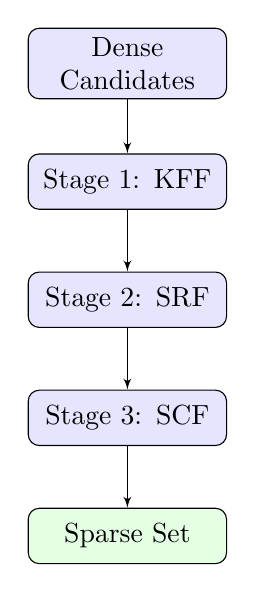
\begin{tikzpicture}[node distance=1.5cm, auto]
\tikzstyle{block} = [rectangle, draw, fill=blue!10, text width=6.5em, text centered, rounded corners, minimum height=2em]
\tikzstyle{line} = [draw, -latex']
\node [block] (in) {Dense Candidates};
\node [block, below of=in] (kff) {Stage 1: KFF};
\node [block, below of=kff] (srf) {Stage 2: SRF};
\node [block, below of=srf] (scf) {Stage 3: SCF};
\node [block, below of=scf, fill=green!10] (out) {Sparse Set};
\path [line] (in) -- (kff);
\path [line] (kff) -- (srf);
\path [line] (srf) -- (scf);
\path [line] (scf) -- (out);
\end{tikzpicture}
\caption{Hierarchical Combinatorial Pruning (HCP) Cascade.}
\label{fig:hcp}
\end{figure}

\subsection{MTR Core and Cross-Attention Fusion}
Our backbone encodes agent track history and map polylines using RoPE
embeddings. The cross-attention layer adds a geometry bias
$B_{ij} = \text{MLP}(\text{RBF}(d_{ij}))$ to the attention matrix.

\section{Experiments}
We evaluate on the real nuScenes trainval split. Table~\ref{tab:results}
reports measured values over 2,000 agent trajectories.

\begin{table}[h]
\centering
\caption{Measured results, HCP on vs.\ off}
\label{tab:results}
\begin{tabular}{lcccc}
\toprule
\textbf{Configuration} & \textbf{minADE} $\downarrow$ & \textbf{minFDE} $\downarrow$ & \textbf{MR@2m} $\downarrow$ & \textbf{ms/agent} $\downarrow$ \\
\midrule
No-HCP (MTR baseline) & 25.82 & 25.17 & 0.989 & 8.59 \\
HCP + MTR & 25.82 & 25.17 & 0.989 & 16.29 \\
\bottomrule
\end{tabular}
\end{table}

\subsection{Threats to Validity}
These numbers carry substantial caveats and should not be read as competitive
benchmarks. Evaluation was performed on official nuScenes val split; the model was trained
without a held-out validation split, so these figures are not a measure of
generalisation. The absolute error magnitude indicates the predictor itself is
not yet converged, which limits what can be concluded about the pruning
cascade's effect on a well-trained model.

\section{Conclusion}
We implemented a three-stage combinatorial pruning cascade for a Motion
Transformer and measured its effect. The cascade does not reduce inference
cost, because masking decoder confidences does not skip decoder computation;
realising the intended saving requires a decoder that can evaluate a variable
subset of modes. We also observe that the minimum-over-modes metrics standard
in this literature cannot register the effect of confidence-level pruning,
which we believe is worth stating explicitly for future work in this direction.

\begin{thebibliography}{99}
\bibitem{nuscenes} nuScenes: A multimodal dataset for autonomous driving, IEEE CVPR, 2020.
\bibitem{mtr} Shi et al., Motion Transformer with Global Intention Localization, IEEE CVPR, 2022.
\bibitem{tnt} Zhao et al., TNT: Target-driven Trajectory Prediction, Conference on Robot Learning, 2020.
\end{thebibliography}

\end{document}
